\documentclass[12pt, titlepage]{article}
\usepackage{geometry}
\usepackage{graphicx}
\usepackage{siunitx}

\geometry{legalpaper, margin=1in}
\renewcommand{\figurename}{Slika}
\renewcommand{\contentsname}{Sadržaj}

\title{\textbf{Upravljački algoritmi u realnom vremenu \\ Projekat 3 - \textit{Pump Station}}}
\date{Jun 29., 2023.}
\author{\textit{Kandidati}: Nenad Radović, Djordje Ristić, Petar Popov, Filip Stevanović \\ \textit{Profesor}: Zeljko Kanović}

\begin{document}
    \maketitle
    \thispagestyle{empty}
    \newpage

    \tableofcontents
    \thispagestyle{empty}
    \newpage
    
    \section{\textbf{Opis sistema}}

        \subsection{Elementi sistema}

            Sistem koji pokušavamo regulisati sastoji se od:

            \begin{enumerate}
                \item \textbf{Regulacionog ventila $Y_1$}, kojim se dovodi tečnost u rezervoar.
                \item \textbf{Pumpe $P_1$ i $P_2$}, kojima se ispumpava dovedena tečnost iz rezervoara.
                \item \textbf{Senzori $B_1$, $B_2$, $B_3$, $B_4$ i $B_5$}, koji su binarni senzori i daju naznaku
                o dostignutom nivou tečnosti.
            \end{enumerate}

        % Ovdje ide slika sistema

            \begin{figure}[ht]
                \centering
                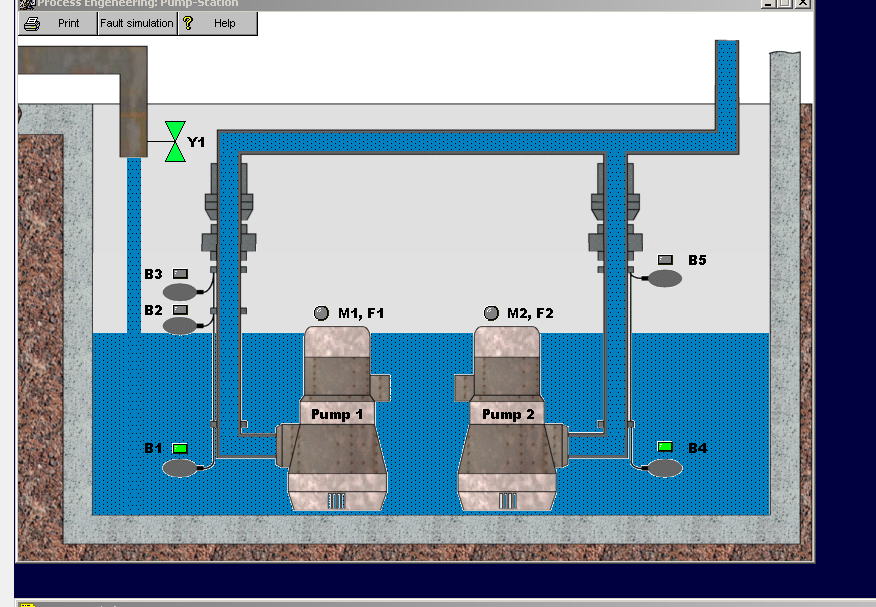
\includegraphics[width=\textwidth]{Slike/SYSTEM APPEARANCE.PNG}
                \caption{\textit{Izgled sistema}}
            \end{figure}
        
        % Ovdje ide slika upravljačke table

        \subsection{Opis rada sistema}

            \subsubsection{Automatski režim rada}

                Pretpostavimo da je u rezervoaru (prije uključivanja sistema) postojao odredjen nivo 
                tečnosti i da je taj nivo iznad senzora $B_1$ i $B_4$ (dakle, ti senzori
                će davati signal aktivacije, a pošto su \textbf{normalno otvoreni}, davaće logičku jedinicu -
                baš kao na slici iznad).
                Neka je, takodje, ventil $Y_1$ koji pušta tečnost u rezervoar \textbf{otvoren}, u početnom trenutku.

                Ako aktiviramo automatski režim rada, sistem \textbf{neće reagovati} (pri pretpostavljenim početnim uslovima)
                sve dok ne dodje do aktivacije senzora $B_2$, koji je takodje \textbf{normalno otvoren}. 
                Kada izlaz pomenutog senzora postane logička jedinica, u tom trenutku automatski režim aktivira jednu od pumpi
                (podrazumijevano je da aktivira pumpu $P_1$). 

                Po uslovu zadatka, ako je nivo tečnosti u bilo kojem vremenskom trenutku aktivirao senzor $B_2$ ali nije
                $B_3$, potrebno je da pumpe \textbf{rade naizmjenično} sve dok se tečnost ne spusti iznad senzora $B_1$ ili $B_4$.
                To je ostvareno tajmiranjem vremena rada pumpi, gdje svaka ima pravo da radi maksimalno $30$ sekundi,
                osim ako se ne desi ikakva promjena u sistemu.

                Kada jedna pumpa nije sama sposobna da ispumpava tečnost iz rezervoara, dolaziće do rasta nivoa 
                tečnosti - samim time i do aktivacije senzora $B_3$. Ako senzor $B_3$ da naznaku da je do njega došla tečnost,
                tada se \textbf{bezuslovno aktiviraju obje pumpe} sve dok nivo tečnosti ne padne ispod senzora $B_1$ ili $B_4$.

                Ekstreman slučaj u sistemu predstavlja prejak dotok i prebrzo punjenje rezervoara, te obje pumpe
                nisu dovoljno moćne da ispumpavaju tečnost iz sistema. U tom slučaju, tečnost će rasti sve do senzora 
                $B_5$, a kada je on aktiviran, daće naznaku upravljačkom sistemu da zatvori ventil $Y_1$, te 
                će obje pumpe nastaviti sa radom sve dok nivo tečnosti ne padne ispod senzora $B_1$ ili $B_4$.

            \subsubsection{Ručni režim rada}

                Ručni režim rada ostvaruje se preklopom prekidača \textit{Hand/Auto} sa \textit{Auto} na \textit{Hand}.
                Tada je isključivo moguće mijenjati stanja pumpi pomoću dugmadi \textit{Pumps ON} i \textit{Pumps OFF}.
                
                Ako se stisne dugme \textit{Pumps ON}, ono daje naznaku aktivacije obje pumpe, te one kreću sa 
                ispumpavanjem tečnost iz rezervoara. Obratnu funkciju vrši prekidač \textit{Pumps OFF}.

                Potrebno je paziti na rad pumpi "na suvo", te je u tu svrhu dodat "stražar" pod nazivom \textit{Hand Error},
                koji neće dozvoliti paljenje pumpi ako je nivo tečnost ispod detekcije senzora $B_1$ ili $B_4$.
            
    \section{\textbf{\textit{LabView} kod za regulaciju sistema}}

        \textit{LabView} programska podrška za regulaciju opisanog sistema koncipirana je iz nekoliko dijelova:

        \begin{enumerate}
            \item \textbf{Dio aplikacije na računaru} predstavlja nadzorno-upravljački sistem kojim se daju komande
            za regulisanje sistema, medju kojima su prethodno navedene funkcionalnosti - 
            \textbf{prebacivanje iz automatskog u ručni režim i obratno}, \textbf{uključivanje i isključivanje pumpi}, 
            \textbf{uključivanje i isključivanje regulacionog sistema u automatskom režimu}, kao i \textbf{ukazivanje na i otklanjanje greške}.
            \item \textbf{Dio aplikacije na \textit{cRIO} modulu} predstavlja modul koji prima komande sa računara,
            adekvatno ih interpretira te daje parametre za regulaciju sistema (prebacivanje iz jednog stanja u drugo i sl.).
        \end{enumerate}

        \subsection{\textbf{Dio aplikacije na računaru}}

            Dio aplikacije na računaru zadužen je za davanje komandi koje kontrolišu sistem.
            \textit{VI} na kojem se nalazi upravljački \textit{front panel} nalazi se u fajlu \textit{SCADA.vi}.
            Pored pomenutog \textit{.vi} fajla nalazi se još jedan "pomoćni" fajl, nazvan \textit{MIDDLE.vi}, 
            čija funkcionalnost će biti objašnjena kasnije.

            \begin{figure}[ht]
                \centering
                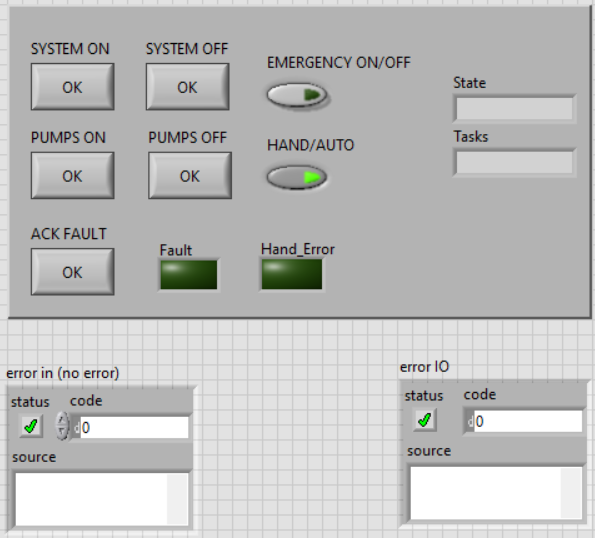
\includegraphics[width=0.55\textwidth]{Slike/SCADA.vi FRONT PANEL.png}
                \caption{\textit{Upravljački Front Panel}}
            \end{figure}

            \textbf{Upravljačka tabla} se tako sastoji od nekoliko elemenata:

            \begin{enumerate}
                \item \textbf{\textit{Hand}/\textit{Auto} prekidač}, kojim se bira željeni režim rada - \textbf{ručni} i \textbf{automatski}.
                \item \textbf{\textit{System ON} / \textit{System OFF} dugmad}, koji isključivo
                imaju funkcionalnost u automatskom režimu rada i čijim se pritiscima daje naznaka da li postoji
                automatska regulacija ili ne.
                \item \textbf{\textit{Pumps ON} / \textit{Pumps OFF} dugmad}, koji isključivo
                imaju funkcionalnost u ručnom režimu rada i čijim se pritiscima daje naznaka da li je omogućen
                rad pumpi ili ne.
                \item \textbf{\textit{Emergency OFF} dugme}, čijom aktivacijom ili deaktivacijom dajemo 
                naznaku da je došlo do greške u sistemu ili da smo "svjesni" te doznake, respektivno.
                \item \textbf{\textit{Acknowledge Fault} dugme}, na čiji pritisak se "oslobadjamo", odnosno
                otklanjamo grešku u sistemu.
            \end{enumerate}

            Kod koji pomaže pri realizaciji funkcionalnosti sistema "trči" kroz \textit{Timed Loop} strukturu,
            koja je formatirana na izvršavanje na svakih \SI{100}{\ms}. Razlog tome jeste enkapsulacija vremena
            koje je potrebno da senzor da odziv na prisustvo tečnosti, kao i vremena koje je potrebno da 
            signal dodje do upravljačke konzole.
            
            U \textit{Timed Loop} strukturi nalazi se \textit{Event Case} struktura, koja je postavljena 
            da na pritisak proizvoljnog dugmeta reaguje na zahtjev, obradi ga i pošalje adekvatnu 
            komandu \textit{cRIO} modulu, ako je to moguće.

            \begin{figure}[ht]
                \centering
                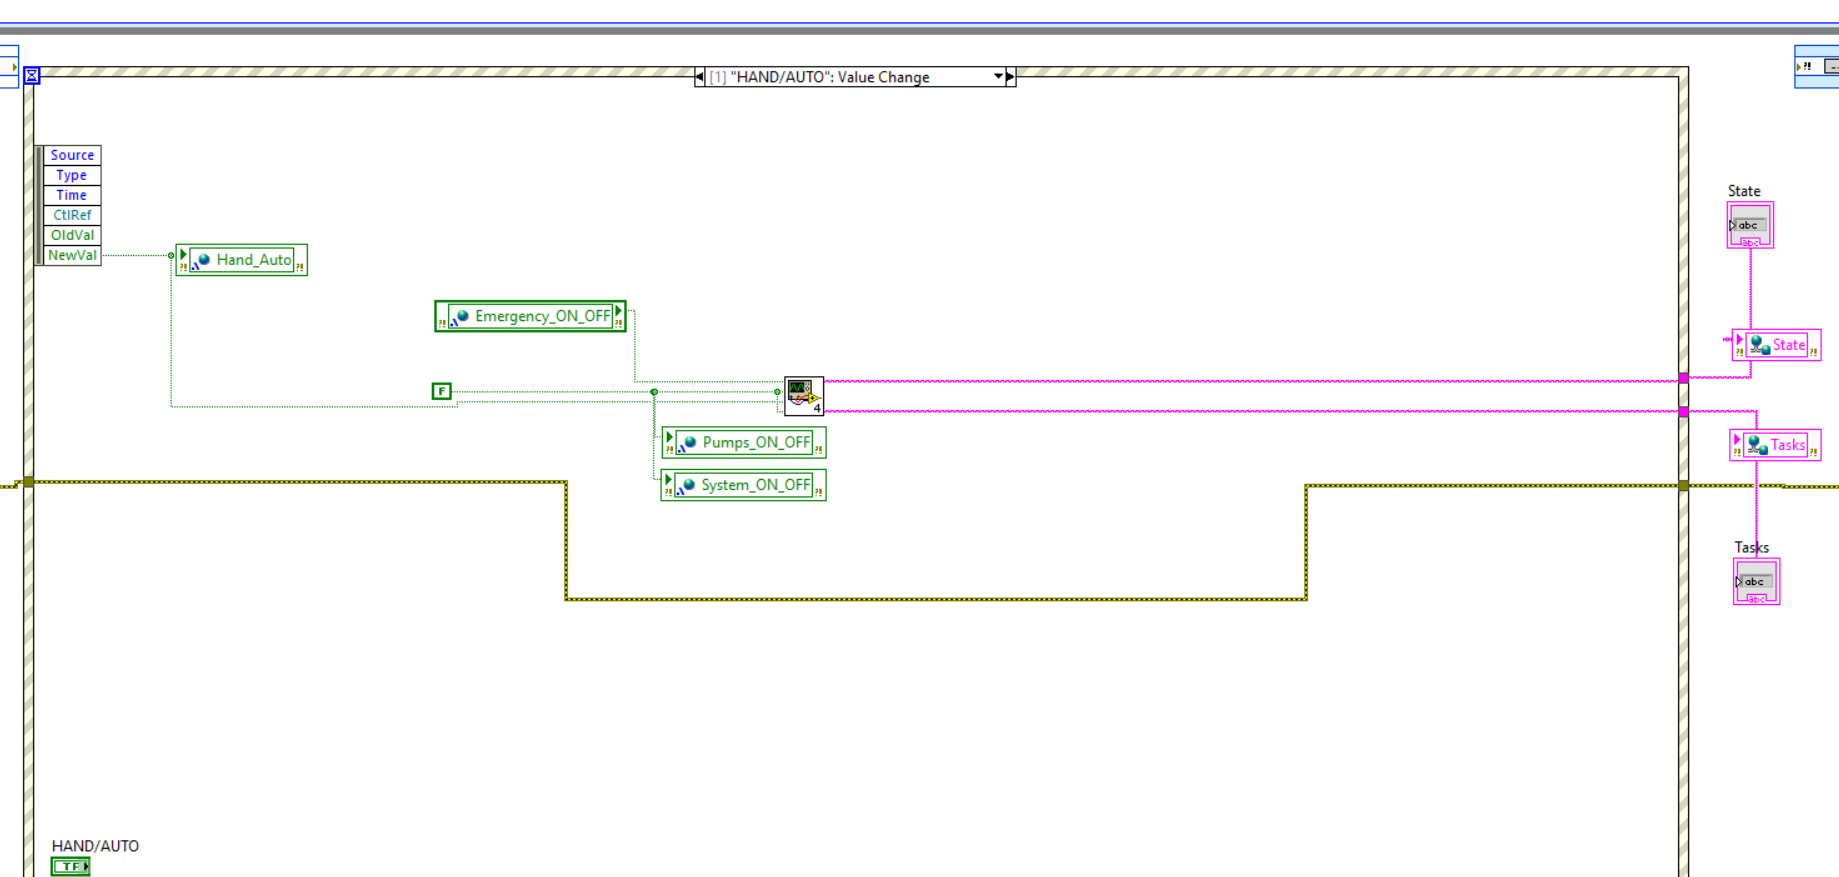
\includegraphics[width=\textwidth]{Slike/SCADA.vi HAND-AUTO CASE.png}
                \caption{\textit{Izgled Event strukture na promjenu Hand/Auto prekidača}}
            \end{figure}

            Promjenljive koje vidimo na slici 3. služe za čuvanje trenutnog stanja sistema, 
            odnosno trenutnog stanja prekidača i dugmadi (recimo, pritisak na \textit{Pumps ON}
            izazvaće promjenu promjenljive \textit{Pumps\_ON\_OFF} na \textit{True} vrijednost,
            dok će pritisak na dugme \textit{Pumps OFF} ovu promjenljivu promijeniti na \textit{False}
            vrijednost - slično i za ostale promjenljive), te se oni prosledjuju pri pozivanju funkcionalnosti \textit{MIDDLE.vi}. 

            \textit{MIDDLE.vi} ima ulogu odlučivanja stanja rada sistema - proizvodi adekvatnu komandu
            na pritisak jednog od dugmadi, ali ne vrši odlučivanje šta se dalje dešava u sistemu, kako se 
            reaguje na senzore i sl. Suštinski, uloga ovog dijela sistema najviše se ogleda
            pri prelazu iz režima u režim.

            \begin{figure}[ht]
                \centering
                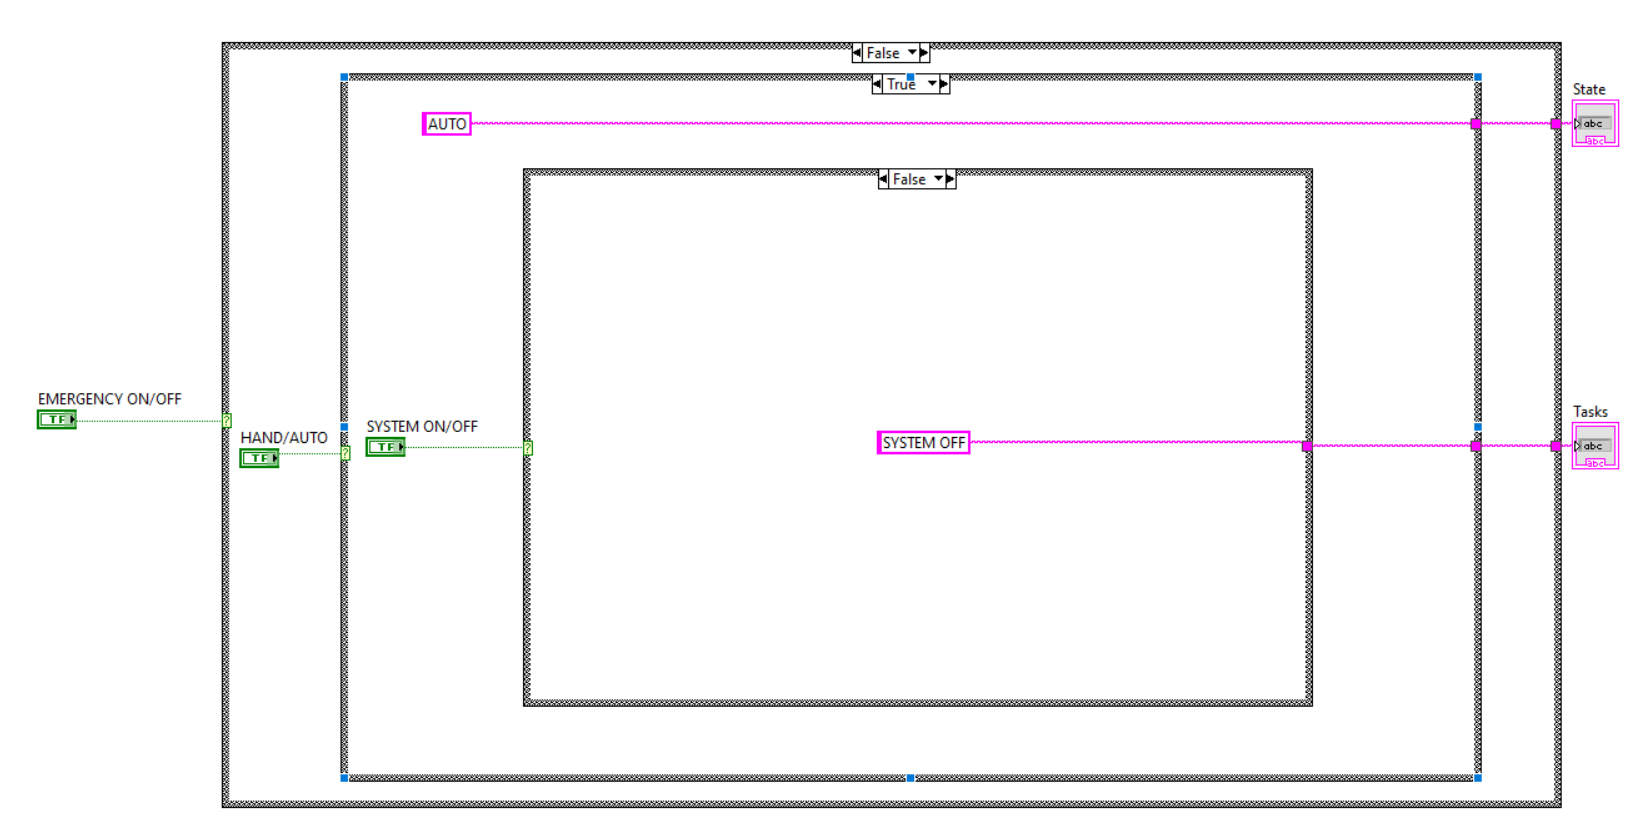
\includegraphics[width=\textwidth]{Slike/MIDDLE.vi CODE.png}
                \caption{\textit{Izgled MIDDLE.vi}}
            \end{figure}
            
            Komande koje se dobijaju iz \textit{MIDDLE.vi} funkcionalnosti prosledjuju se u 
            mrežne promjenljive \textit{State} (koja označava da li bi trebalo da reaguje 
            \textit{Hand}, \textit{Auto} ili \textit{Emergency} dio sistema) i \textit{Tasks} 
            (koja označava koje "zadatke" dobija pomenuti dio sistema).

            Problem koji se može desiti jeste ponovno pritiskanje prethodno pritisnutog dugmeta,
            gdje sistem ne bi trebalo da reaguje jer zapravo nema nove komande. Pomenuti problem se upravo 
            rješava promjenljivima, čije prethodno stanje se provjerava te ako novo nije jednako sa njim,
            prelazi se u obradu komande. 

            Pored toga, u obavezi smo zaustaviti i pogrešno, odnosno nedozvoljeno davanje komandi. 
            Pod time se misli da se komande ograniče na svoj režim - ne možemo davati komande 
            vezane za automatskom režimu ako smo u ručnom režimu, kao i da se komande ne priznaju ako
            smo u \textit{Emergency} slučaju. 

            \newpage

            \begin{figure}[ht]
                \centering 
                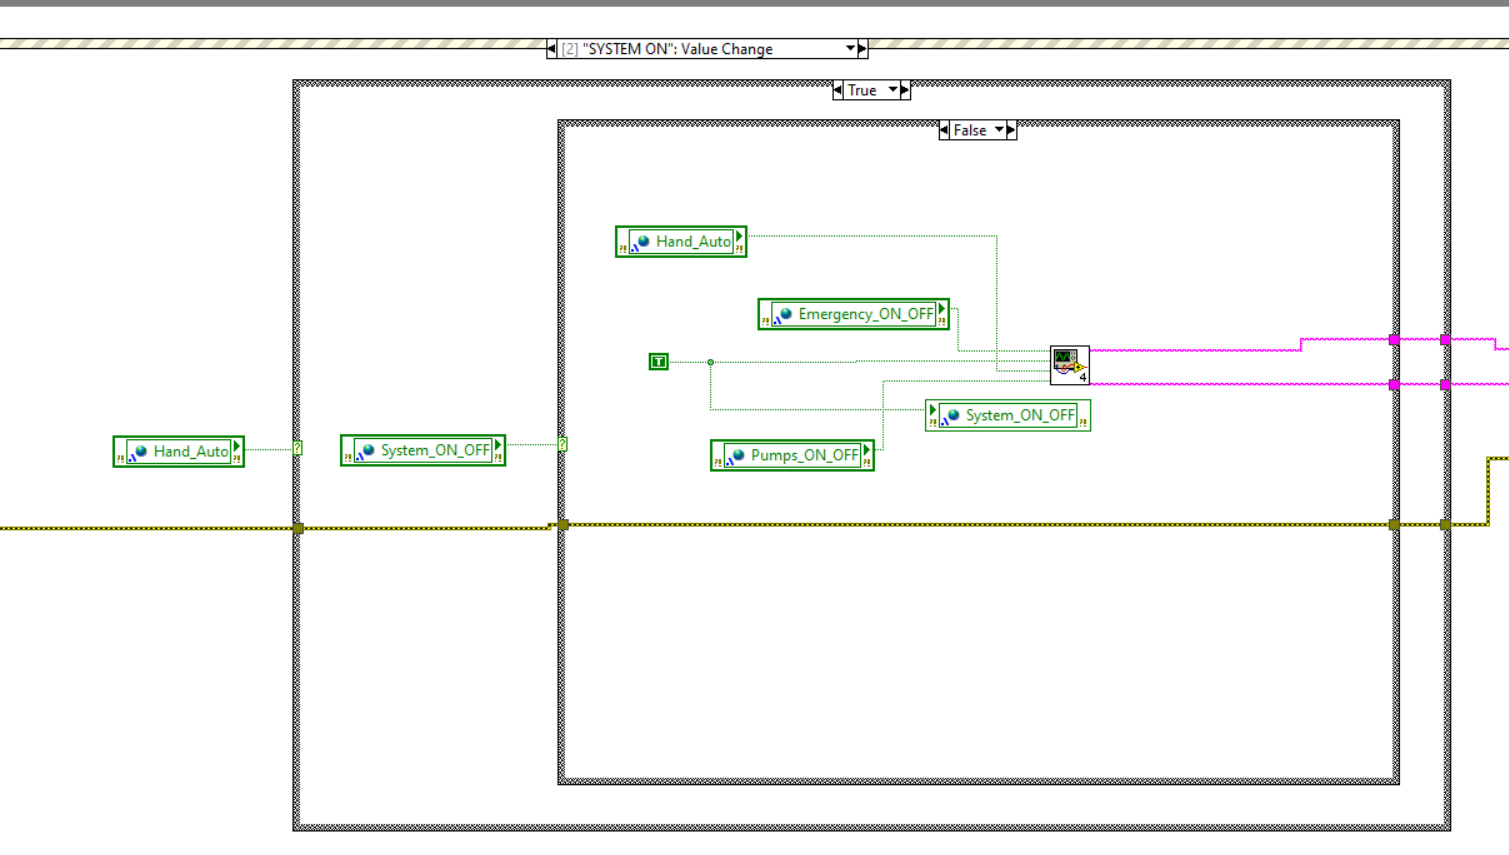
\includegraphics[width=\textwidth]{Slike/SCADA.vi SYSTEM ON CASE.png}
                \caption{\textit{Prikaz slučaja System ON, gdje se provjeravaju uslovi za ispunjenje komande}}
            \end{figure}

            Posebno interesantan slučaj jeste kada je sistem u \textit{Emergency} stanju, te je potrebno
            pored pritiska na dugme koje "nas oslobadja" od takvog stanja stisnuti i 
            dugme \textit{Acknowledge Fault} koje briše grešku iz sistema.

            \begin{figure}[ht]
                \centering 
                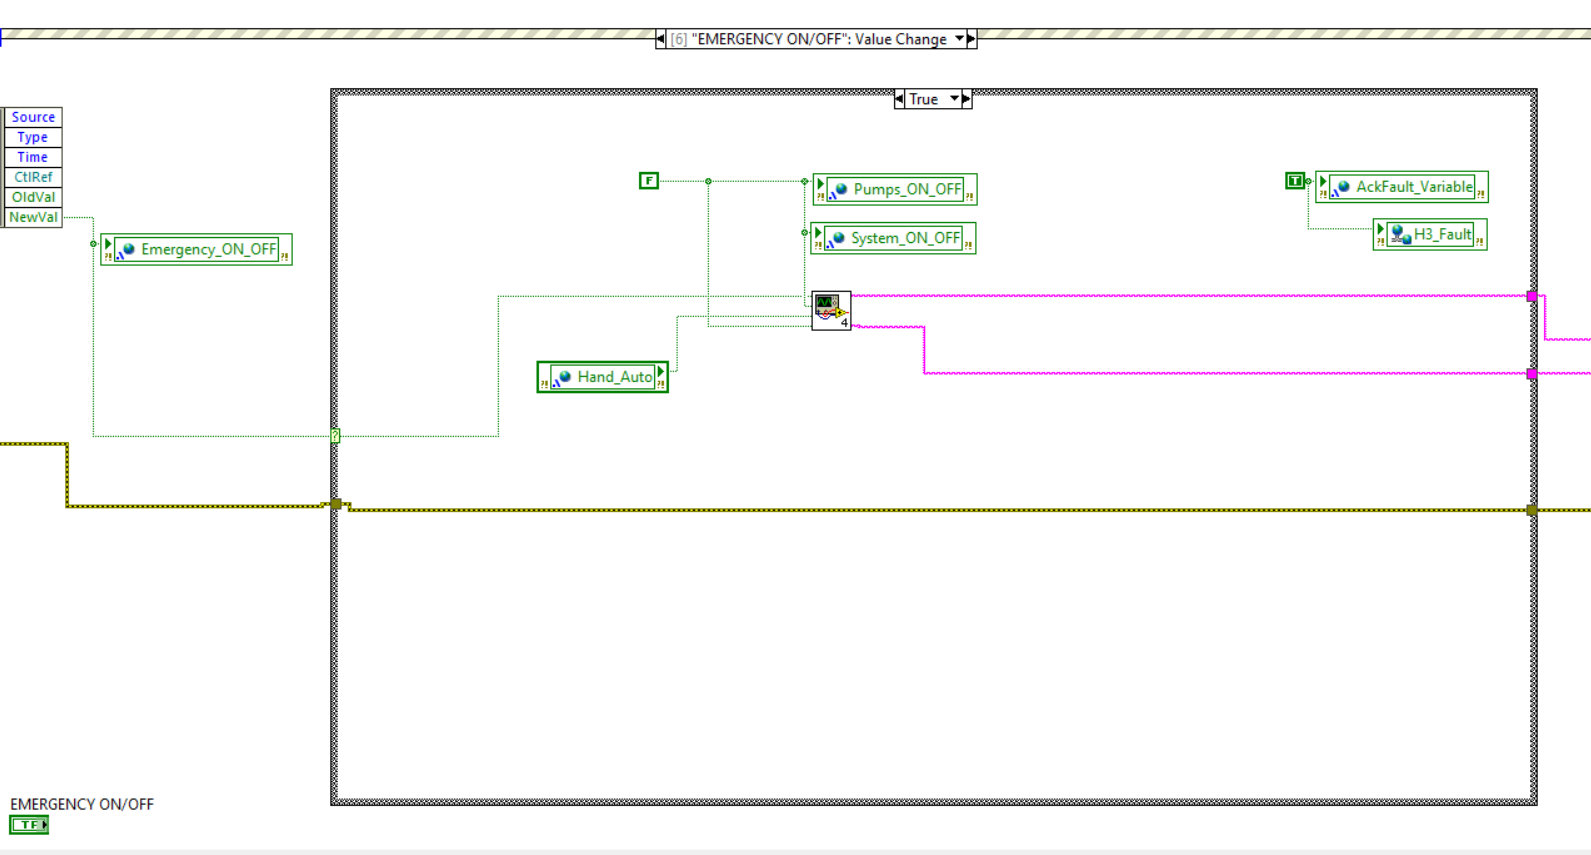
\includegraphics[width=\textwidth]{Slike/SCADA.vi EMERGENCY CASE.png}
                \caption{\textit{Prikaz slučaja Emergency, kada dodje do prekida u radu}}
            \end{figure}

            Uslov da se predje u dalje otklanjanje greške jeste da se prvo vrati \textit{Emergency ON/OFF}
            dugme na \textit{False} vrijednost, te zatim pritisne \textit{Acknowledge Fault} dugme.
            Nakon toga se sistem vraća u stanje koje je prethodilo grešci, ali sa isključenim motorima. 
            Može se smatrati da se sistem "restartuje".

            \newpage

            \begin{figure}[ht]
                \centering
                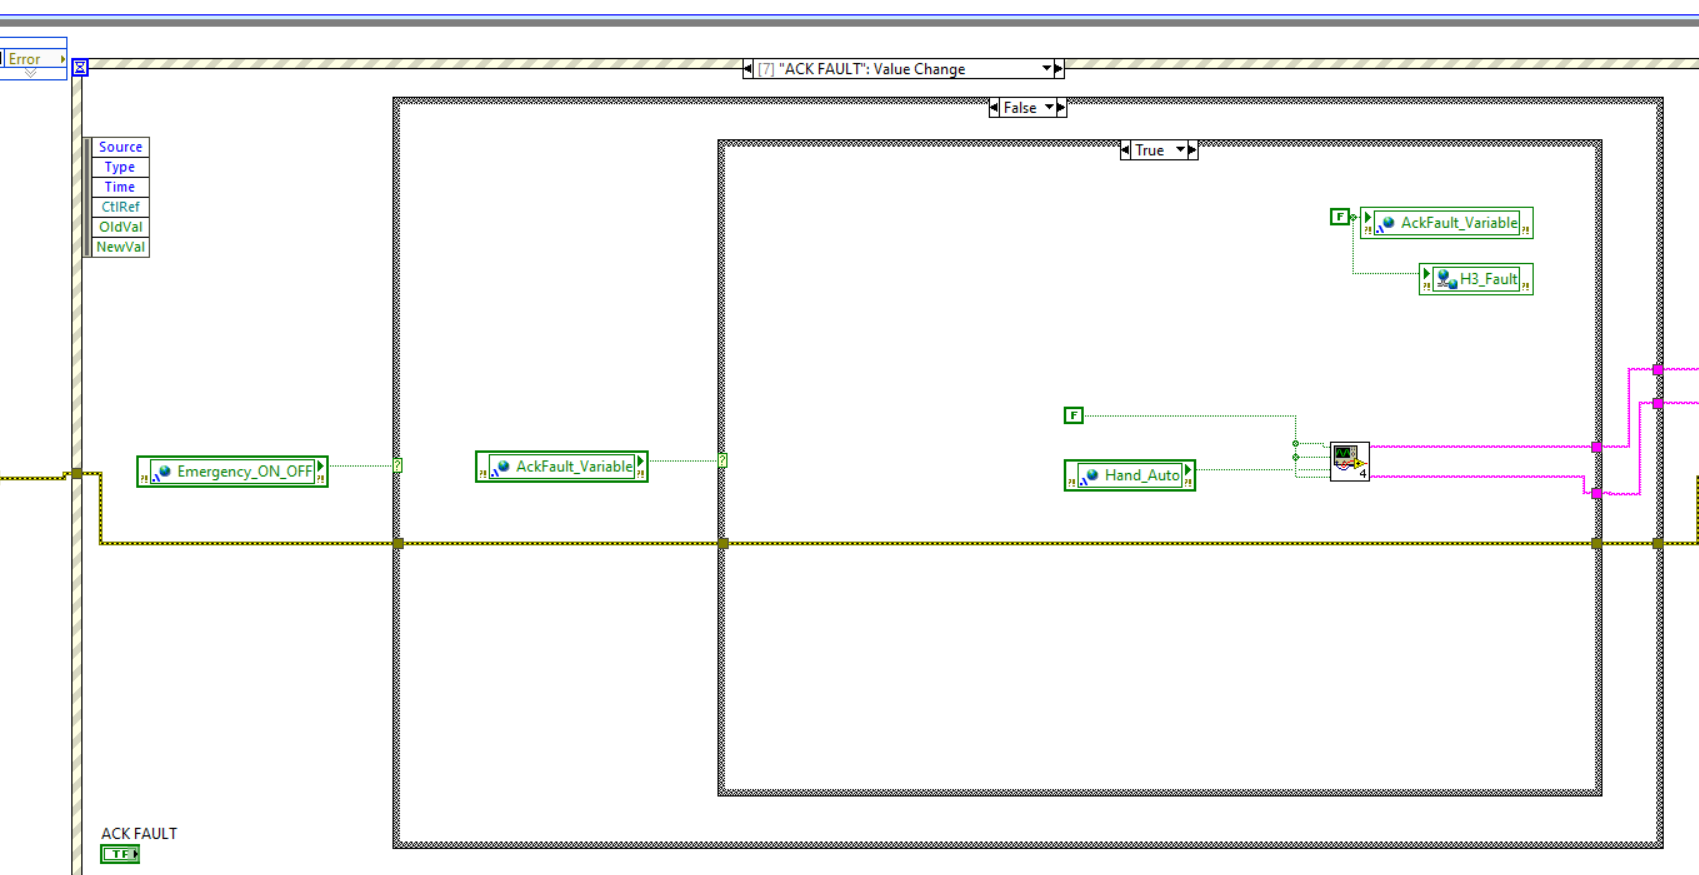
\includegraphics[width=\textwidth]{Slike/SCADA.vi ACK FAULT CASE.png}
                \caption{\textit{Prikaz slučaja kada se pritisne Acknowledge Fault dugme}}
            \end{figure}
        
            Ostali slučajevi su slični po konstrukciji, u smislu razmatranja promjenljivih za svoj rad.
        
        \subsection{\textbf{Dio aplikacije na \textit{cRIO} kontroleru}}
        
            Postoje dva fajla koja se nalaze na \textit{cRIO} kontroleru, a to su 
            \textit{cRIO.vi} i \textit{HAND\_AUTO.vi}.

            \subsubsection{\textit{cRIO.vi}}

                U \textit{cRIO.vi} fajlu vršimo inicijalizaciju jednoprocesnih i mrežnih promjenljivih
                na njihove podrazumijevane vrijednosti, te konstantno prosledjujemo stanje ulaza i izlaza
                sa \textit{cRIO} uredjaja, kao i na \textit{cRIO} uredjaj.

                \textit{Flat Sequence} struktura jeste tu da natjera izvršavanje inicijalizacije promjenljivih 
                prije samog kupljenja njihovih vrijednosti sa ulaza, kao i postavljanja njihovih vrijednosti na 
                izlaze \textit{cRIO} uredjaja.

                \begin{figure}[ht]
                    \centering
                    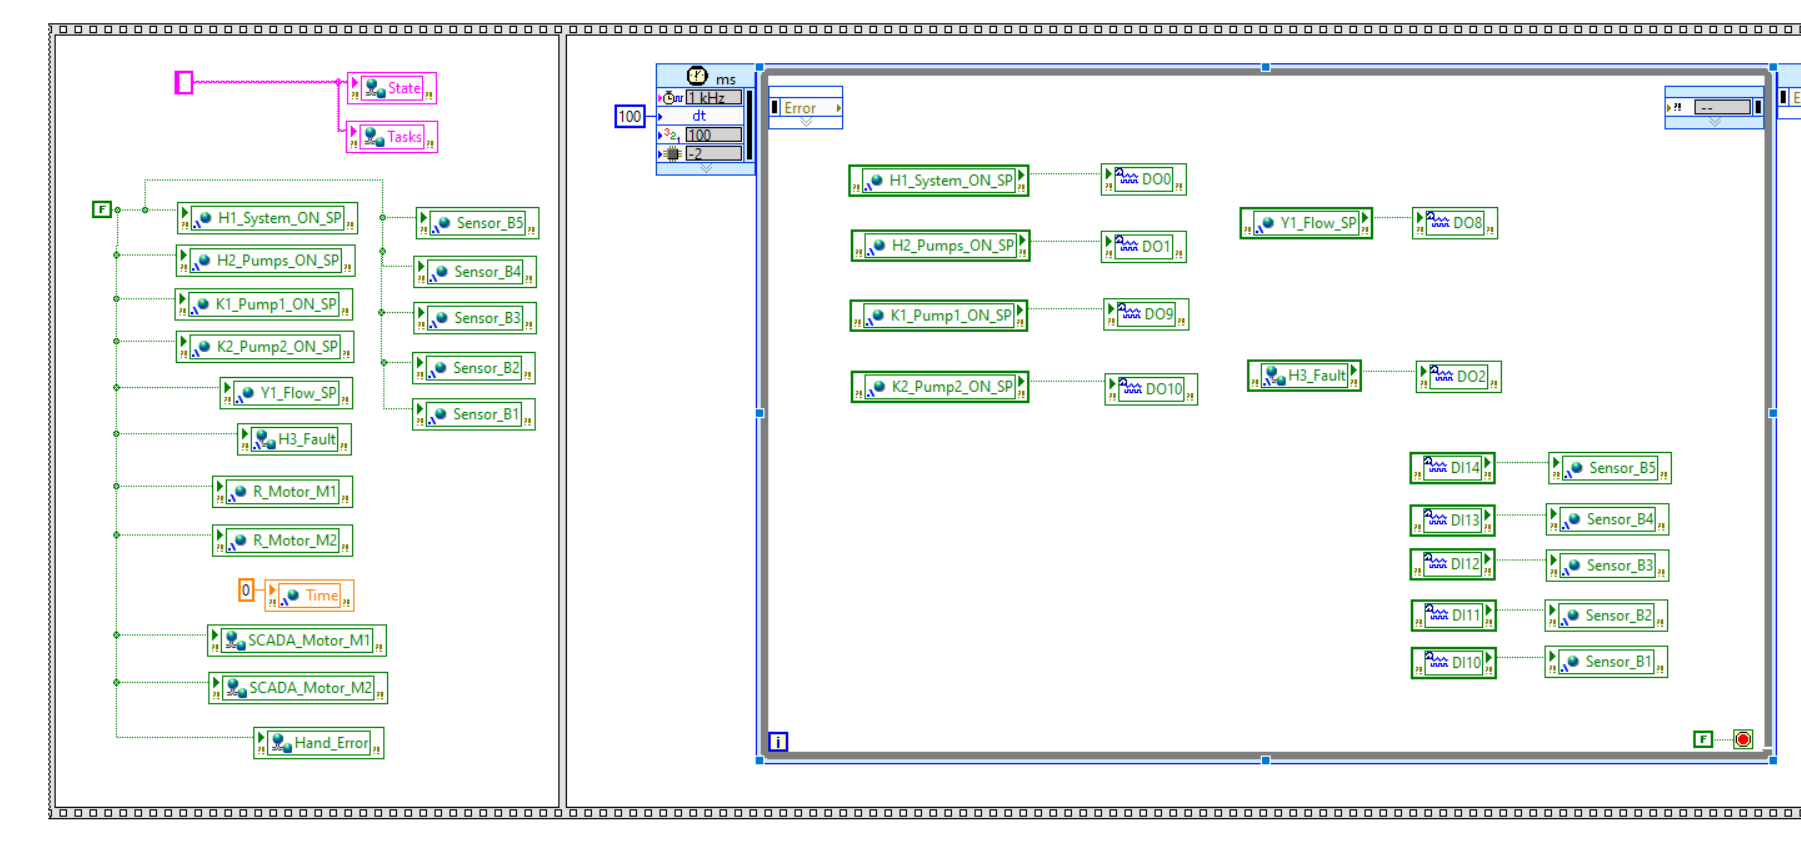
\includegraphics[width=\textwidth]{Slike/cRIO.vi CODE.png}
                    \caption{\textit{Izgled cRIO.vi}}
                \end{figure}

                Razlog postojanja \textit{Timed Loop} strukture isti je kao i u prethodnoj sekciji - enkapsulacija vremena
                kupljenja i postavljanja signala.

                \newpage

            \subsubsection{\textit{HAND\_AUTO.vi}}

                Najinteresantniji dio gdje se odvija čitava logika automatskog i ručnog sistema nalazi se u \textit{HAND\_AUTO.vi} fajlu.
                
                U samom \textit{VI} izvršavaju se dvije \textit{Timed Loop} strukture, gdje jedna vodi glavnu logiku,
                dok druga služi za tajmiranje, o kojem će biti više riječi u nastavku teksta.

                U prvoj petlji smještena je spoljašnja \textit{Case} struktura, koja razlikuje svoje slučajeve
                pomoću mrežne promjenljive \textit{State}, čiji je tip \textit{String} i čiju vrijednost
                mijenjamo direktno u \textit{SCADA.vi}, kao što smo već vidjeli. Pomenuli smo da stanja
                koja može uzeti pomenuta promjenljiva jesu \textbf{\textit{HAND}}, \textbf{\textit{AUTO}} i 
                \textbf{\textit{EMERGENCY}}. 

                Razmotrimo stanje \textbf{\textit{HAND}}. Od značaja dolazi indikator \textit{HAND\textbackslash{}AUTO}, 
                koja govori da li se dešava prelaz sistema iz \textit{HAND} režima u \textit{AUTO} režim.
                Ovo je posebno značajno jer se dešava sledeće:

                \begin{itemize}
                    \item[$-$] Sistemski, prelaz iz stanja \textit{AUTO} u stanje \textit{HAND} je isti  
                    kao prelaz iz \textit{Pumps ON} internog stanja u \textit{Pumps OFF} interno stanje - 
                    u oba slučaja dešava se gašenje pumpi.
                    \item[$-$] Potrebno je razlikovati ta dva slučaja gašenja pumpi jer je 
                    potrebno u slučaju prelaska iz
                    \textit{AUTO} u \textit{HAND} zapamtiti stanje i aktivnost pumpi (zahtjev
                    pri izradi sistema - pumpe "pamte" kakve su bile u \textit{AUTO} režimu).
                    \item[$-$] Uvodi se pomoćna varijabla \textit{HAND\textbackslash{}AUTO}, koja će razlikovati
                    prethodno opisana dva slučaja.
                \end{itemize}

                \begin{figure}[ht]
                    \centering
                    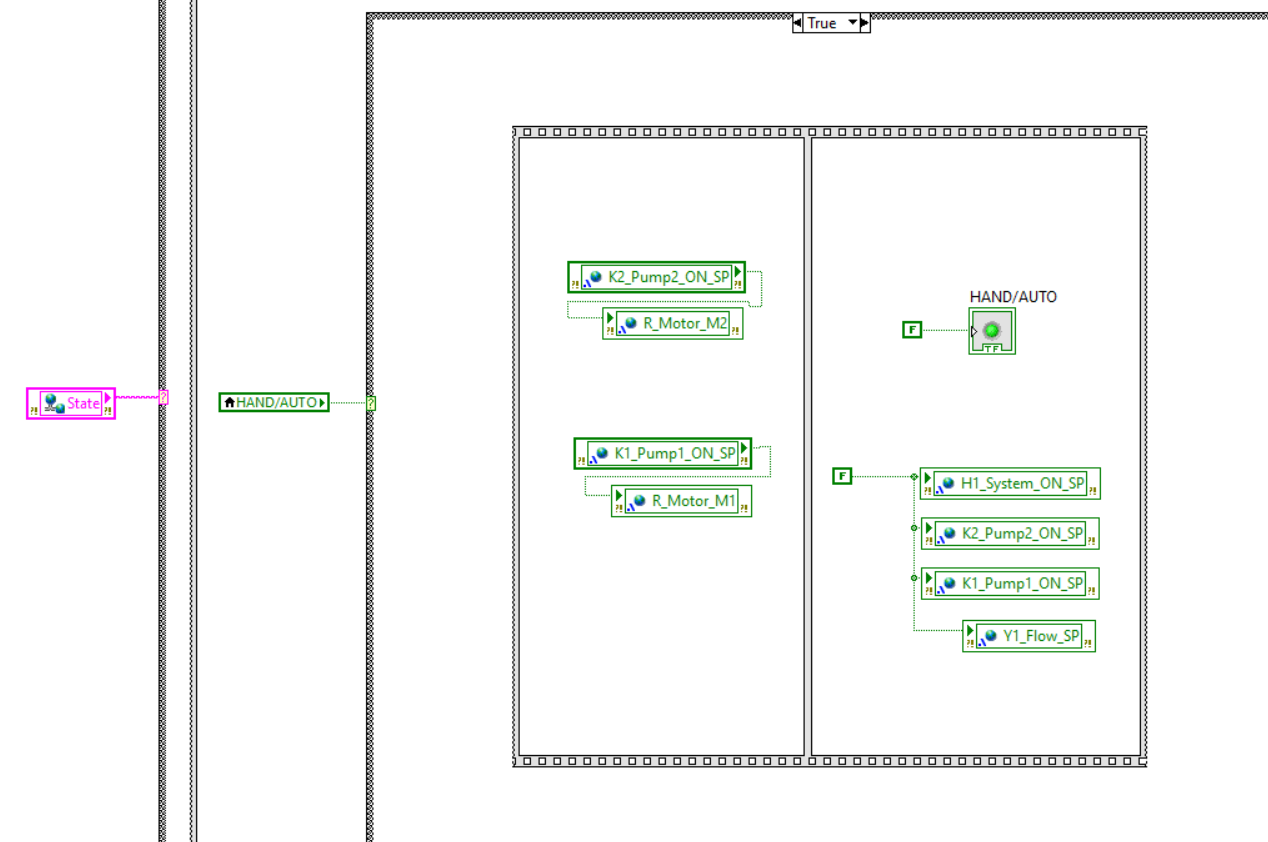
\includegraphics[width=0.73\textwidth]{Slike/HAND_AUTO.vi AUTO TO HAND.png}
                    \caption{\textit{Prelaz iz AUTO u HAND}}
                \end{figure}

                \newpage

                \textit{HAND\textbackslash{}AUTO} bilježi prethodno stanje (uzeto je stanje \textit{True} za automatski,
                kao i \textit{False} stanje za ručni režim), te se tako provjerava da li je došlo do prelaza.
                Kada je to slučaj, indikator se stavlja na vrijednost koja mu odgovara u zavisnosti od režima
                rada, te se vrši pamćenje prethodnog stanja pumpi (za konkretan slučaj sa slike) te gašenje
                istih.

                Ručni režim rada je praktično jednostavan - postoje dvije komande i stanje "čekanja". 
                Ako postoji "zadatak" izdat od upravljačkog dijela sistema, on će se nalaziti u 
                mrežnoj promjenljivoj \textit{Tasks}. 

                Za ručni režim, promjenljiva \textit{Tasks} može uzeti vrijednosti \textit{Pumps ON} i \textit{Pumps OFF}.
                U \textit{Pumps ON} režimu, provjeravamo da li postoji prethodno pomenuta greška, odnosno pad 
                nivoa tečnosti ispod detekcije senzora $B_1$ ili $B_4$. To će odredjivati dozvolu rada pumpi.

                Naravno, kada odradimo zadatak, potrebno je "očistiti" \textit{Tasks} promjenljivu.
                To radimo tako što postavljamo praznu riječ u nju.

                \begin{figure}[ht]
                    \centering
                    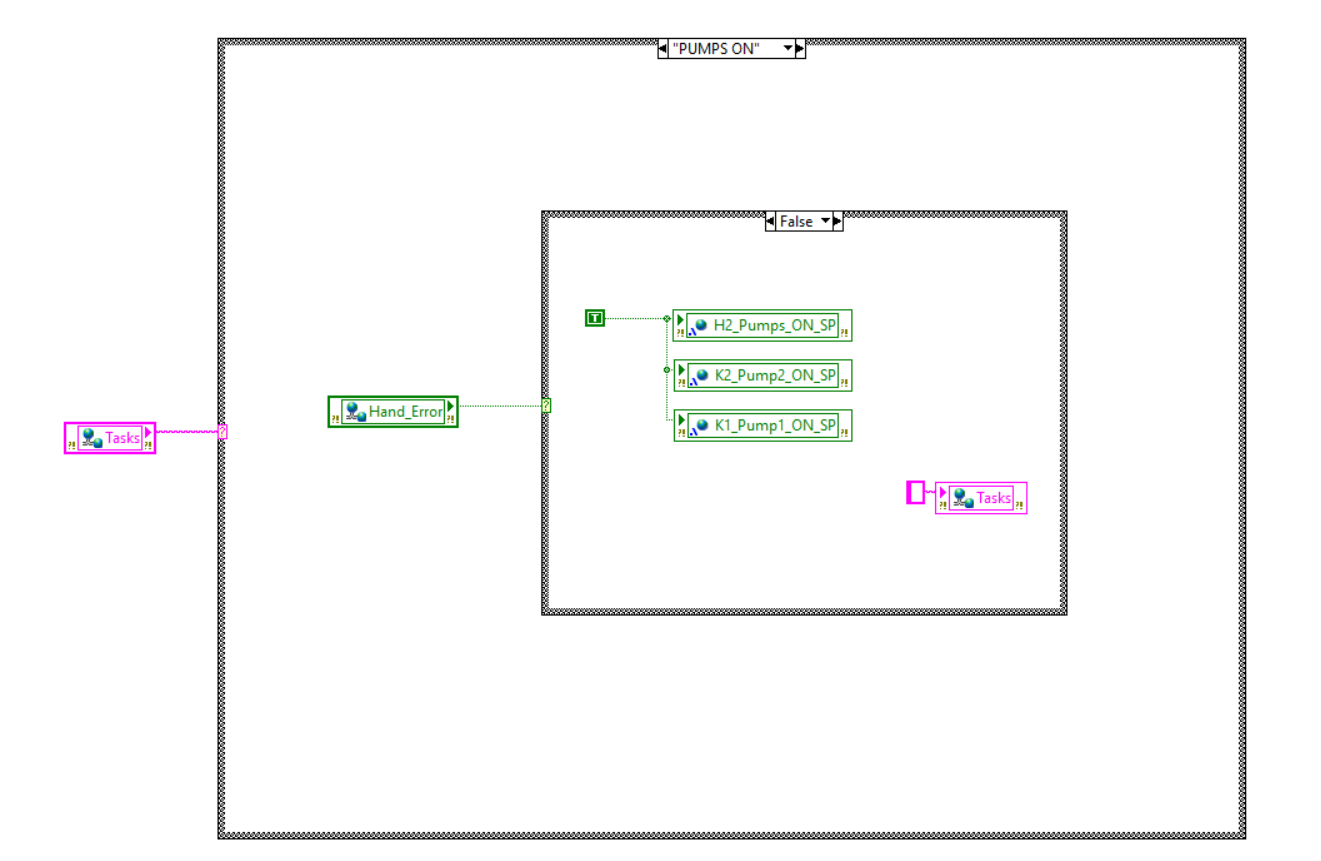
\includegraphics[width=0.9\textwidth]{Slike/HAND_AUTO.vi PUMPS ON.png}
                    \caption{\textit{Pumps ON interno stanje}}
                \end{figure}

                Sličan je rad i \textit{Pumps OFF} internog stanja.

                \begin{figure}[ht]
                    \centering
                    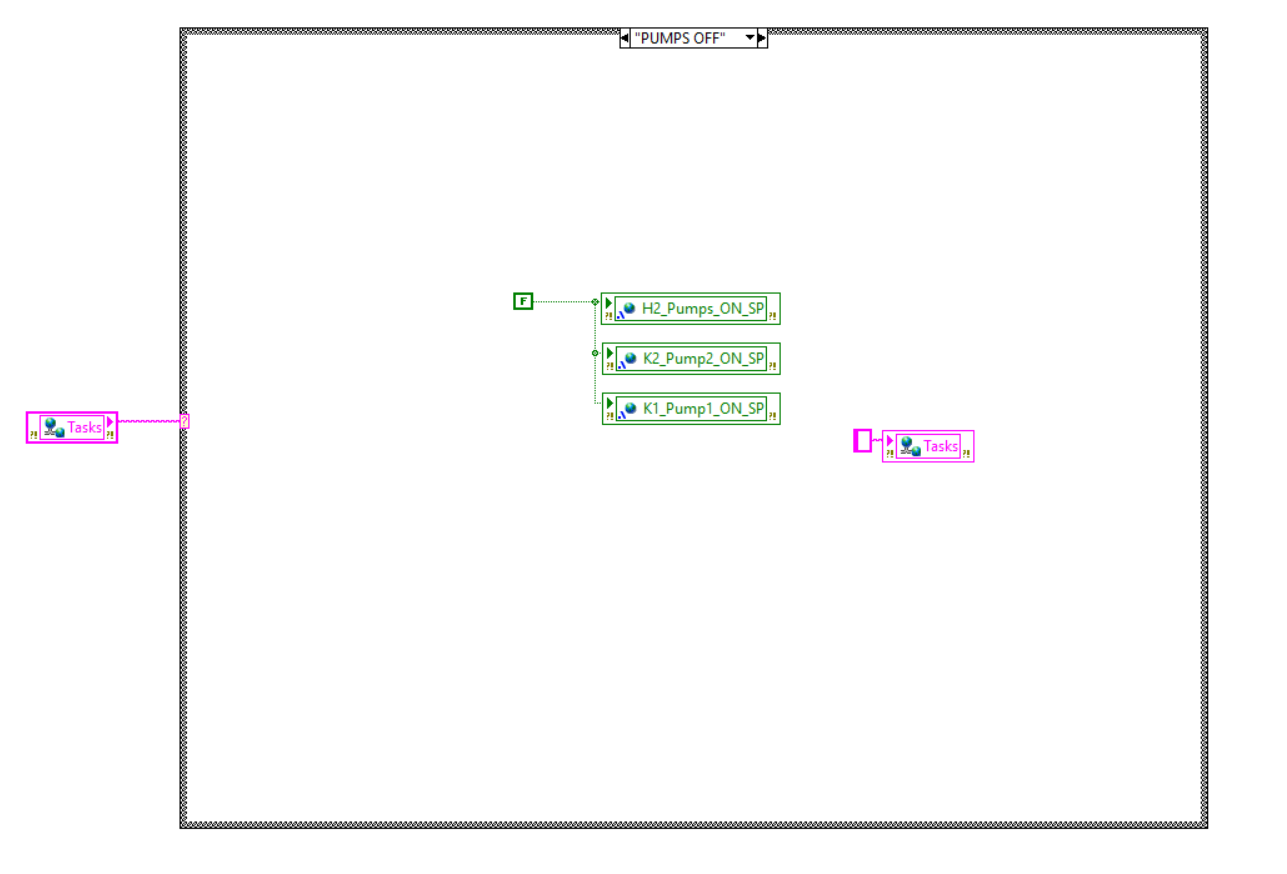
\includegraphics[width=0.9\textwidth]{Slike/HAND_AUTO.vi PUMPS OFF.png}
                    \caption{\textit{Pumps OFF interno stanje}}
                \end{figure}

                Ako promjenljiva sadrži praznu riječ, to je oznaka da se režim postavi u stanje čekanja.
                
                Konkretno za \textit{HAND} režim, čekanje predstavlja posmatranje već pomenutih 
                senzora $B_1$ i $B_4$. Ako nivo tečnosti padne ispod njihove detekcije, dolazi do 
                prestanka rada pumpi - zaštita od rada na suvo. Indikator \textit{Hand Error} se postavlja
                na \textit{True} vrijednost, te se pumpe ne mogu ponovo upaliti sve dok se ne otkloni
                greška.

                Ova greška nije greška za čitav sistem. Naime, potrebno je samo preći u automatski režim rada,
                u kojem je moguće aktivirati ventil $Y_1$ te pustiti tečnost da ponovo napuni rezervoar.

                \begin{figure}[ht]
                    \centering
                    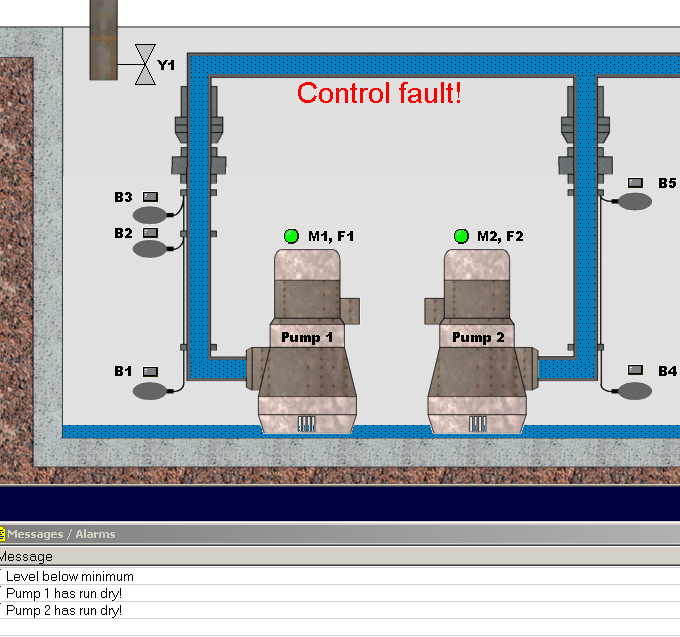
\includegraphics[width=0.7\textwidth]{Slike/HAND DRY PUMPS.PNG}
                    \caption{\textit{Detekcija rada pumpi na suvo}}
                \end{figure}

                \begin{figure}[ht]
                    \centering
                    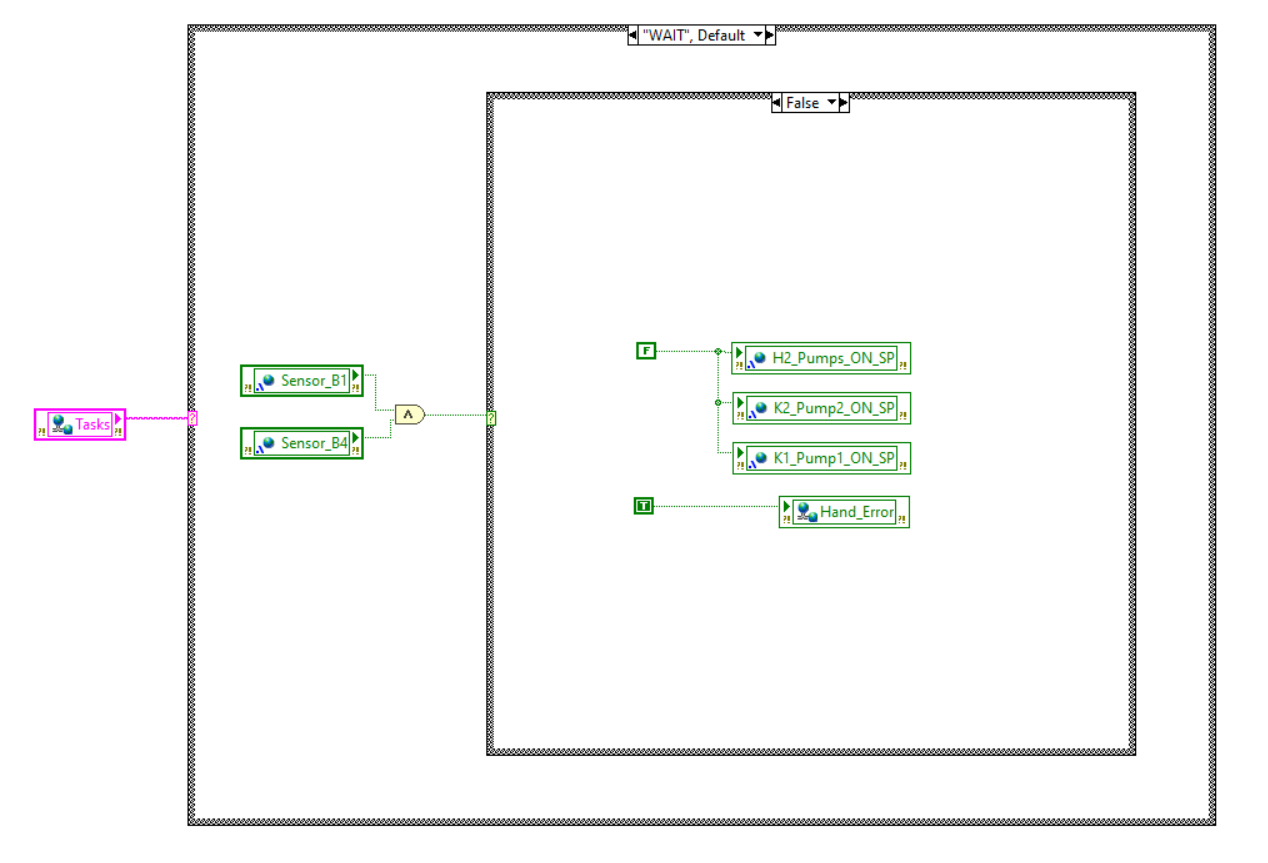
\includegraphics[width=0.9\textwidth]{Slike/HAND_AUTO.vi WAIT.png}
                    \caption{\textit{Interno stanje čekanja - zaštita od rada na suvo}}
                \end{figure}

                \newpage

                Sada ćemo razmotriti stanje \textbf{\textit{AUTO}}. Detekcija prelaska je potrebna i 
                suštinski je ista kao i u \textit{HAND} režimu.

                \begin{figure}[ht]
                    \centering
                    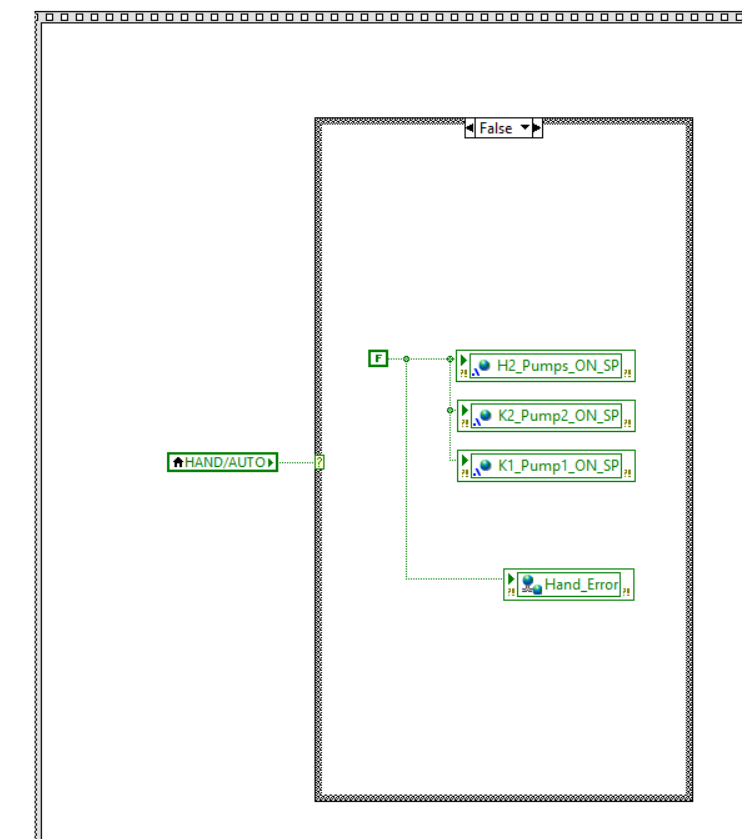
\includegraphics[width=0.5\textwidth]{Slike/HAND_AUTO.vi HAND TO AUTO.png}
                    \caption{\textit{Prelaz iz Hand režima u Auto režim}}
                \end{figure}

                Primjetimo da se otklanja \textit{Hand\_Error} greška jer smo sada u mogućnosti 
                ponovno napuniti rezervoar. Takodje, važno je uvidjeti da ne prebacujemo 
                \textit{HAND\textbackslash{}AUTO} promjenljivu na \textit{True} vrijednost sada -
                razlog tome će ubrzo biti objašnjen.

                Kada smo u automatskom režimu, moguće je alternirati izmedju stanja \textit{System ON}, 
                \textit{System OFF} i \textit{Wait}. Razmotrimo stanje \textit{System OFF}.

                U pomenuto interno stanje se ulazi svaki put kada dodje do prebacivanja u \textit{Auto}
                režim, ili kada se prebacuje iz internog stanja \textit{System ON}, te je ono dužno da ugasi pumpe.
                U tu svrhu uvodimo novu \textit{Case} strukturu, čija istinitost zavisi od logičkog "I"
                dvije promjenljive - \textit{HAND\textbackslash{}AUTO} i negirane \textit{EMERGENCY} 
                promjenljive.

                Naime, ako je \textit{HAND\textbackslash{}AUTO} promjenljiva bila na \textit{False} 
                vrijednosti, dešava se prelaz sa \textit{Hand} režima u \textit{Auto} režim,
                te je potrebno prebaciti pomenutu promjenljivu na \textit{True} vrijednost.
                Takodje, otkanja se greška (ako je postojala). 

                \begin{figure}[ht]
                    \centering
                    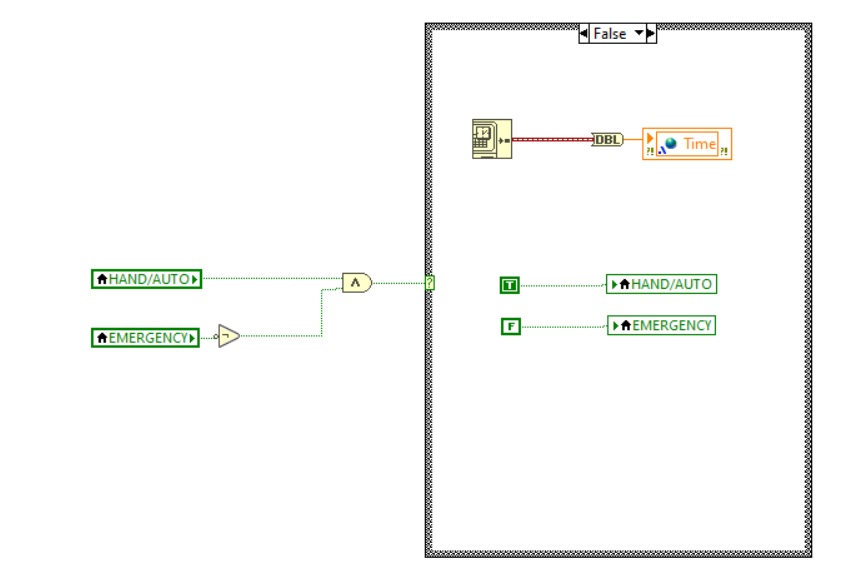
\includegraphics[width=0.7\textwidth]{Slike/HAND_AUTO.vi AUTO SYSTEM OFF 1.png}
                    \caption{\textit{System OFF kada dodje do prelaska izmedju režima}}
                \end{figure}

                Medjutim, ako se desilo da je \textit{HAND\textbackslash{}AUTO} promjenljiva bila na 
                \textit{True} vrijednosti, kao i da nije postojala greška u sistemu, 
                to znači da smo došli iz \textit{System ON} internog stanja, pa je potrebno
                zapamtiti koja od pumpi je radila. 

                \newpage

                \begin{figure}[ht]
                    \centering
                    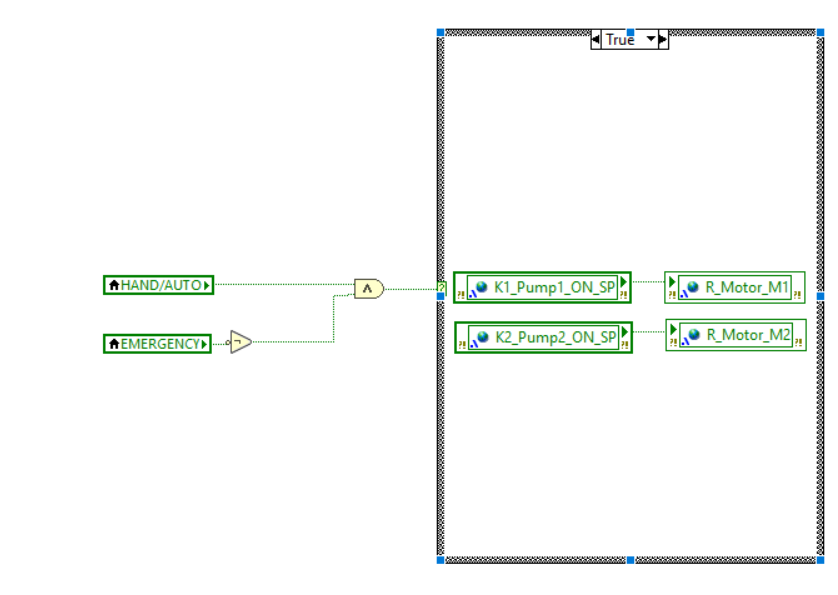
\includegraphics[width=0.7\textwidth]{Slike/HAND_AUTO.vi AUTO SYSTEM OFF 2.png}
                    \caption{\textit{System OFF kada dodje do prelaska izmedju internih stanja}}
                \end{figure}

                \textit{System ON} slučaj je vrlo jednostavan - dolazi do paljenja pumpi (odnosno prepisivanja
                zapamćenog stanja).

                \begin{figure}[ht]
                    \centering
                    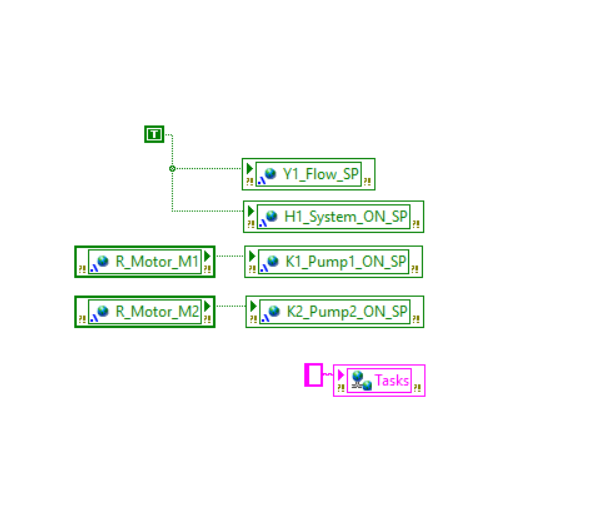
\includegraphics[width=0.7\textwidth]{Slike/HAND_AUTO.vi AUTO SYSTEM ON.png}
                    \caption{\textit{System ON interno stanje}}
                \end{figure}

                Slučaj gdje se čitava automatska regulacija odvija jeste stanje čekanja - \textit{Wait} 
                interno stanje. Ono prati logiku dešavanja opisanu u pasusu $1.2.1$, dok se njegova 
                realizacija sastoji od mnoštvo \textit{Case} struktura koje zavise od 
                provjere aktivnosti senzora.

                Kreće se od provjere da li je sistem za regulaciju uključen, što se nalazi u 
                \textit{H1\_System\_On\_SP} promjenljivoj. Pristup ide "od dole ka gore" - prvenstveno se 
                provjerava aktivnost donjih senzora. Kao što je i opisano, ako jedan od senzora 
                $B_1$ ili $B_4$ ne detektuje prisustvo tečnosti, daje se signal gašenja pumpama, ali se 
                otvara ventil $Y_1$.

                Zanimljivo za razmatrati jeste slučaj kada se nivo vode nalazi izmedju detekcije senzora 
                $B_1$ ($B_4$) i $B_2$. Mi tada nismo sigurni da li tečnost ni u jednom momentu nije došla 
                do senzora $B_2$, ili je došla, ali zbog rada ispumpavanja spustila. Medjutim, ako je tečnost
                već posjetila senzor $B_2$, bar jedna od pumpi će biti upaljena, te ćemo tako razlikovati
                prethodno pomenuta dva slučaja. U tu svrhu koristimo logičko "NILI" kolo, čija tabela izgleda kao

                \newpage

                \begin{figure}[ht]
                    \centering
                    \begin{tabular}{|c|c|c|}
                        \hline
                        \textbf{Pumpa 1 - aktivnost} & \textbf{Pumpa 2 - aktivnost} & \textbf{Rezultat operacije} \\
                        \hline
                        Pumpa nije upaljena (0) & Pumpa nije upaljena (0) & Nismo nikako došli do senzora $B_1$ (1) \\
                        \hline
                        Pumpa je upaljena (1) & Pumpa nije upaljena (0) & Već smo bili do senzora $B_1$ (0) \\
                        \hline
                        Pumpa nije upaljena (0) & Pumpa je upaljena (1) & Već smo bili do senzora $B_1$ (0) \\
                        \hline
                        Pumpa je upaljena (1) & Pumpa je upaljena (1) & Već smo bili do senzora $B_1$ (0) \\
                        \hline
                    \end{tabular}
                    \caption{\textit{Logička reprezentacija opisanog slučaja}}
                \end{figure}

                \begin{figure}[ht]
                    \centering
                    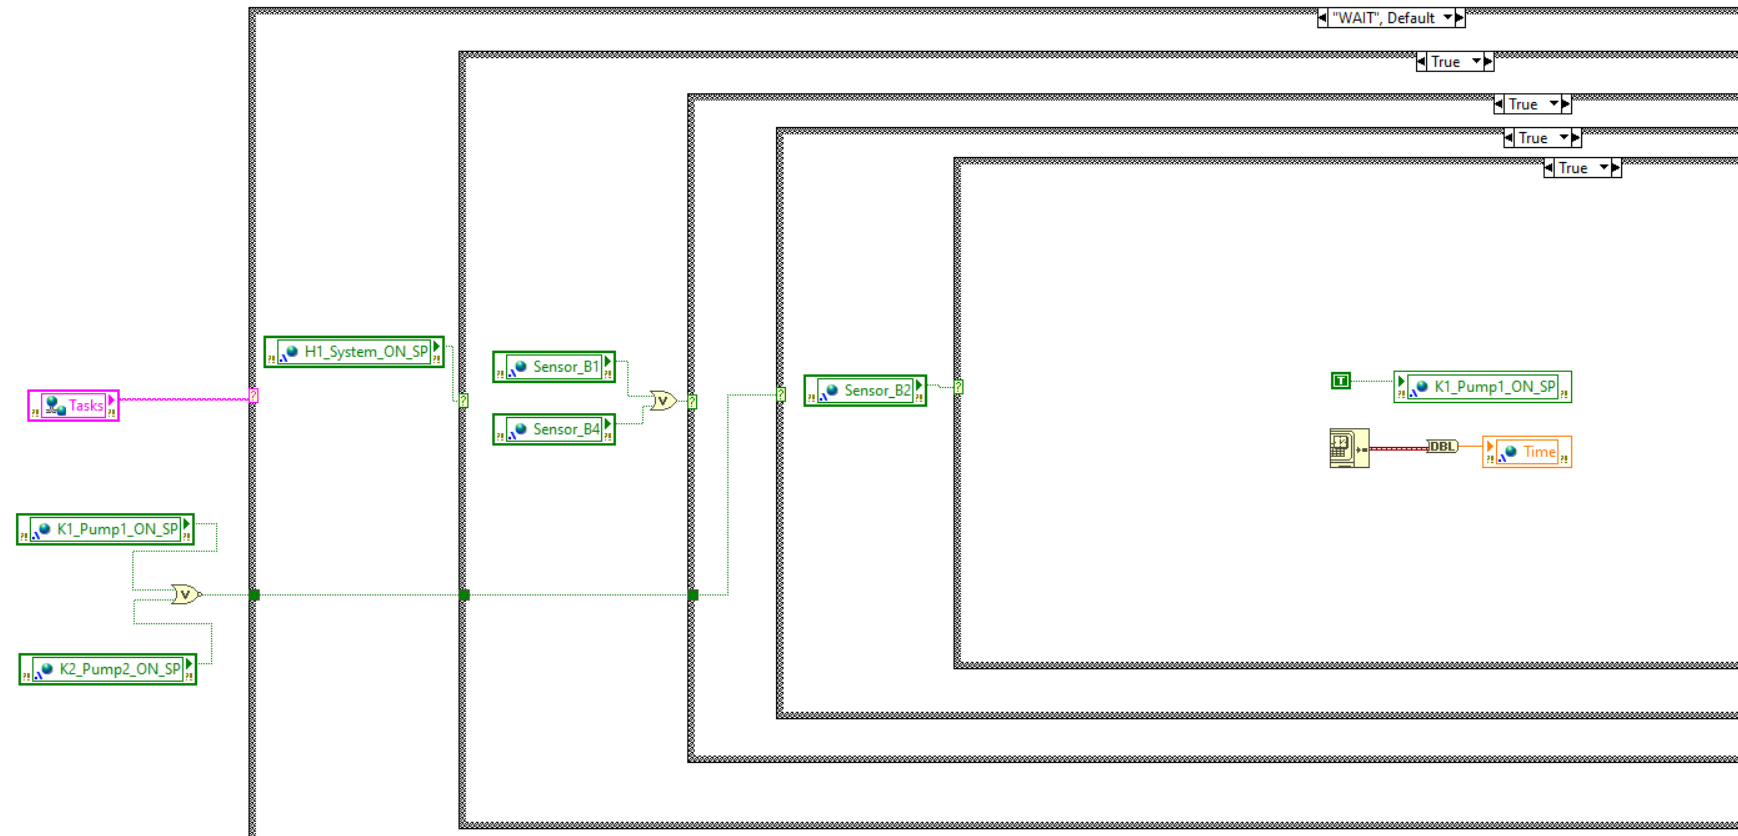
\includegraphics[width=\textwidth]{Slike/HAND_AUTO.vi AUTO WAIT NOSENSORB2.png}
                    \caption{\textit{Slučaj kada tečnost nijednom nije bila na senzoru $B_2$}}
                \end{figure}

                Pričali smo o tome da je potrebno da pumpe rade naizmjenično. Takva naizmjeničnost izvedena je 
                zapisivanjem vremena početka rada jedne pumpe u promjenljivu \textit{Time}, te provjerom da li je prošlo dovoljno vremena
                da se pumpe "zamijene". Provjera se vrši oduzimanjem od trenutnog vremena i ako je ta razlika 
                veća od zadatih sekundi smjene, dolazi do aktivacije indikatora \textit{TIME}. Tajmer "trči" 
                u zasebnoj \textit{Timed Loop} strukturu, kako bi paralelno radio sa ostatkom automatskog sistema.

                \begin{figure}[ht]
                    \centering
                    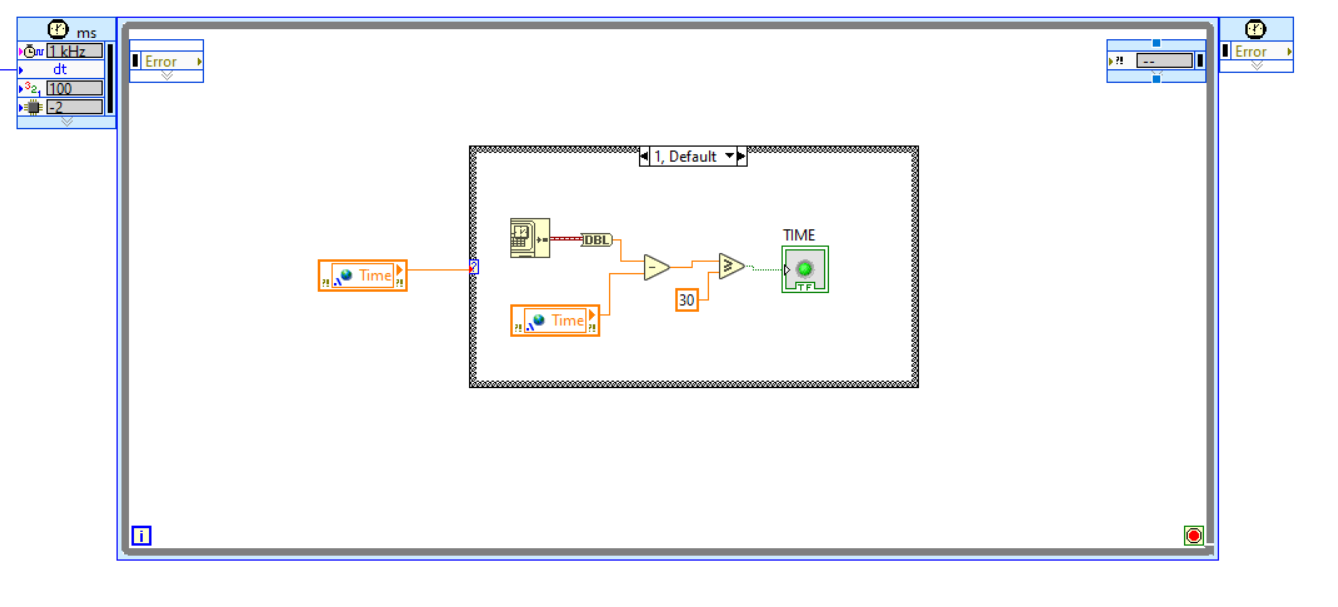
\includegraphics[width=\textwidth]{Slike/HAND_AUTO.vi TIME.png}
                    \caption{\textit{Provjera vremena}}
                \end{figure}

                Naravno, potrebno je da pri naizmjeničnom radu pazimo da li je došlo do aktivacije 
                senzora $B_3$. Ako nije, provjeravamo da li je indikator \textit{TIME} aktiviran, 
                te u skladu sa time mijenjamo rad pumpi. 

                \newpage 

                \begin{figure}[ht]
                    \centering
                    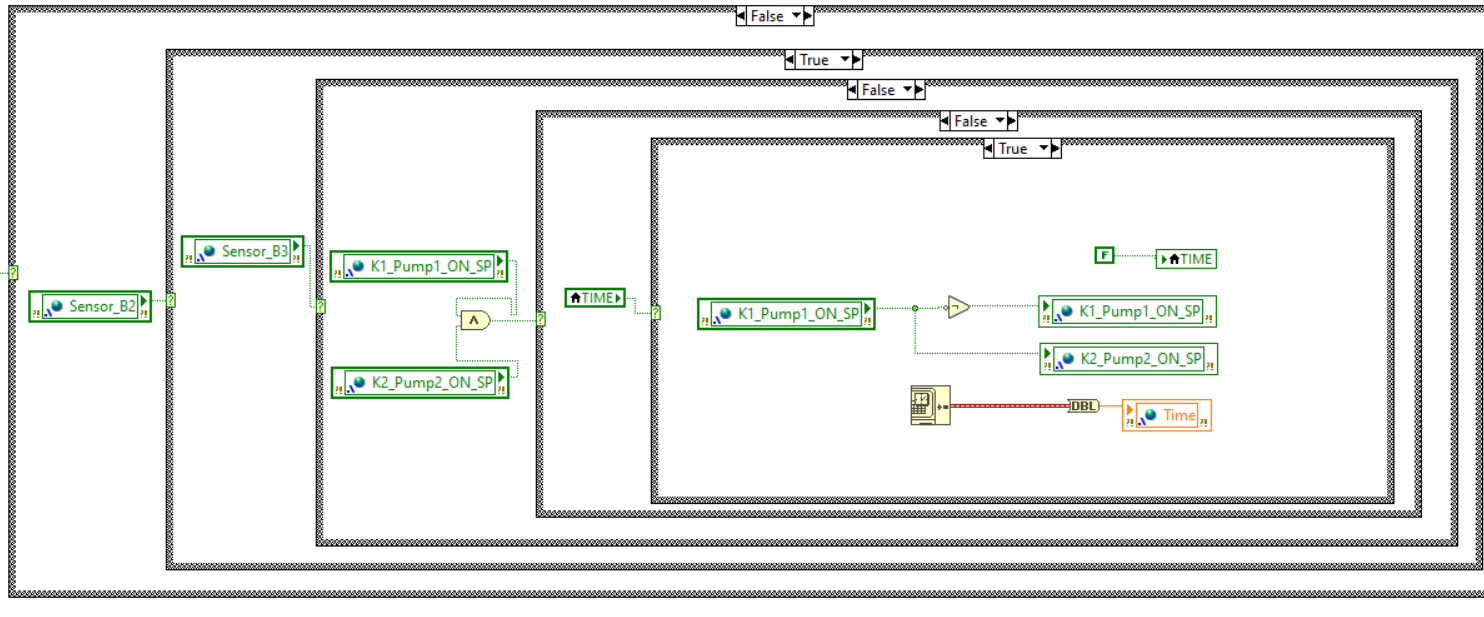
\includegraphics[width=\textwidth]{Slike/HAND_AUTO.vi AUTO PUMP SWITCH.png}
                    \caption{\textit{Naizmjeničan rad pumpi ostvaruje se invertovanjem stanja}}
                \end{figure}

                Važno je napomenuti da se inverzija rada pumpi radi i kada se tečnost nalazi izmedju
                detekcije senzora $B_2$ i $B_3$. Kod i logika za pomenuto su isti.

                Ako je pak došlo do aktivacije senzora $B_3$, obje pumpe kreću sa radom, te se provjerava
                da li je tečnost dostigla i nivo $B_5$ - ako jeste, zatvara se regulacioni ventil i pušta se 
                totalno pražnjenje rezervoara. 

                \begin{figure}[ht]
                    \centering
                    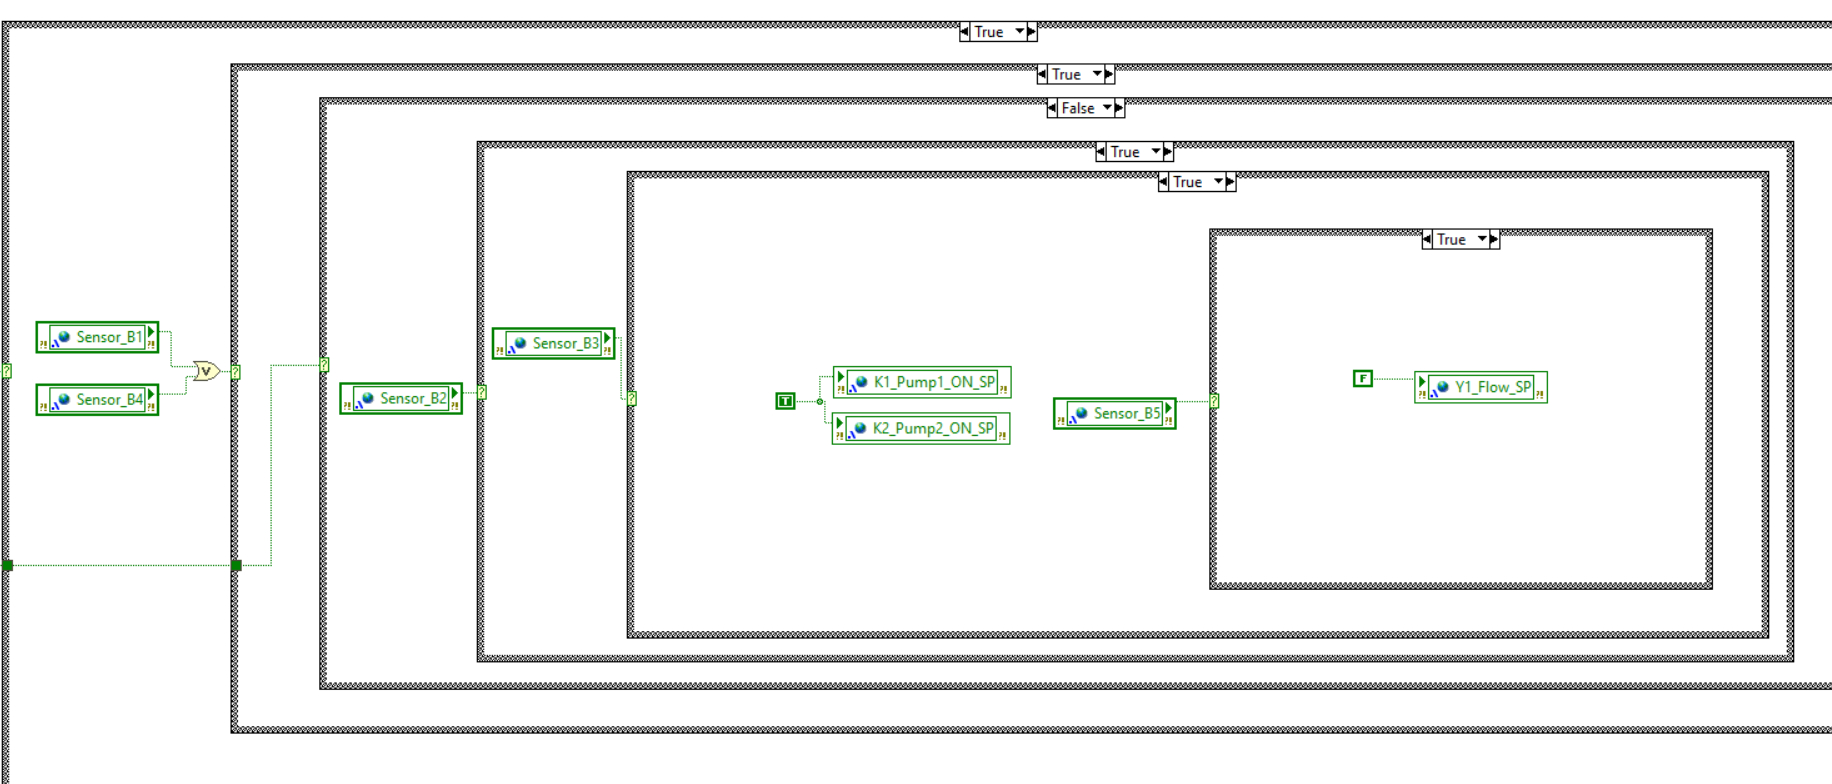
\includegraphics[width=\textwidth]{Slike/HAND_AUTO.vi SENSORB3B5.png}
                    \caption{\textit{Reagovanje na aktivaciju senzora $B_3$ i $B_5$}}
                \end{figure}

                Sistem automatske regulacije radi kontinualno, provjeravajući stanje senzora i kotirajući se po tome.

                \newpage

                Poslednje stanje koje je potrebno razmotriti jeste \textit{Emergency} stanje.
                Kao što je i očekivano, stanje je dužno da ugasi sve pumpe i zapamti prethodna dešavanja 
                u sistemu. Takodje, bitno je da se ne vrši konstantno pamćenje stanja jer će "prava memorija"
                sistema biti izbrisana, te u tu svrhu se uvodi slična logička provjera kao kod prelaza u 
                automatskom režimu. 

                \begin{figure}[ht]
                    \centering
                    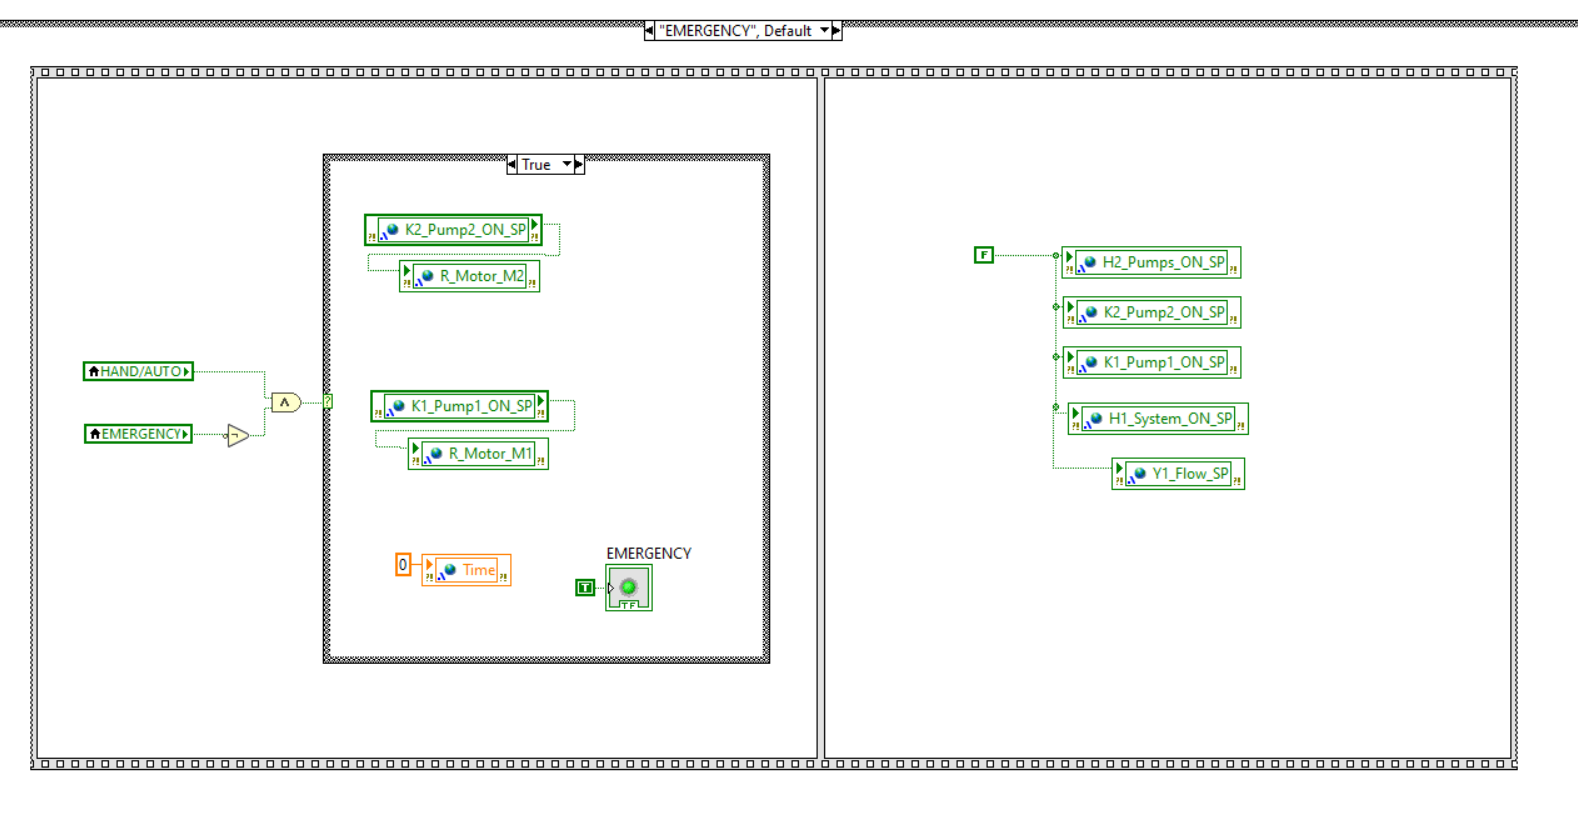
\includegraphics[width=\textwidth]{Slike/HAND_AUTO.vi EMERGENCY.png}
                    \caption{\textit{Emergency slučaj}}
                \end{figure}

                Takodje, potrebno je postaviti vrijednost promjenljive \textit{Time} na $0$,
                što će u drugoj petlji izazvati gašenje tajmera koji ne bi trebalo bespotrebno da broji 
                dok se sistem nalazi u \textit{Emergency} stanju.

                \begin{figure}[ht]
                    \centering
                    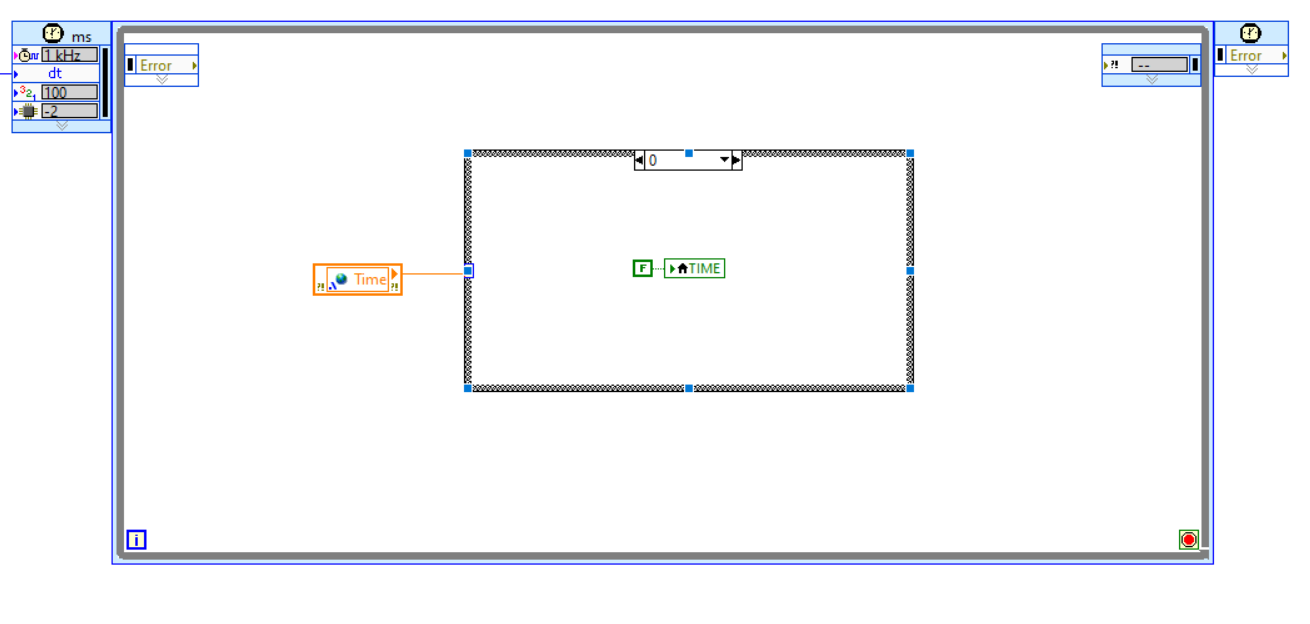
\includegraphics[width=\textwidth]{Slike/HAND_AUTO.vi TIME FALSE.png}
                    \caption{\textit{Gašenje tajmera}}
                \end{figure}
                

\end{document}